\documentclass{beamer-control}
\usepackage{beamer-control-singlefile}
\INCLUDEONLY{Stabilisation by State Feedback}
\begin{document}
\CONCEPT{Stabilisation by State Feedback}

\begin{SUMMARY}
\begin{itemize}
\item State feedback structure
\item Reachable canonical form
\item Eigenvalue assignment
\end{itemize}
\vfill References:
\begin{itemize}
\item \astrom{§7.2}
\end{itemize}
\end{SUMMARY}



\SUBCONCEPT{State feedback structure}

\begin{frame}{Controller structure}
\begin{itemize}
\item We will assume we have a system with a linear state model that has a single input for control
\item How do we design the dynamics of a system through feedback of the state
\item The goal of a feedback controller is to control the output state $y$ to a desired state given by the input $r$
\end{itemize}
\begin{figure}
	\centering
	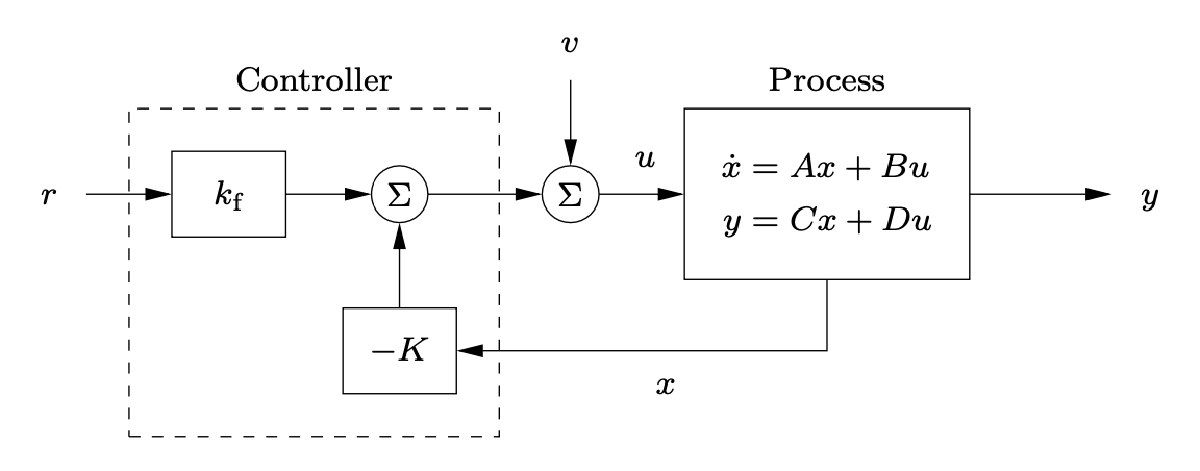
\includegraphics[width=0.8\linewidth]{figure7.5}
	\\
	\textbf{Figure 7.5:} A feedback control system with state feedback.
\end{figure}
\end{frame}


\begin{frame}{Controller structure}
	\begin{itemize}
		\item Consider a system described by
		\[ \frac{\mathrm{d} x}{\mathrm{d} t}=A x+B u, \quad y=C x+D u\]
		\item A linear control law dependent on the state $x$ and reference input $r$ can be given by 
		\[u = -Kx + k_f r\] 
		giving the closed loop state space representation 
		\[\frac{\mathrm{d} x}{\mathrm{d} t} = (A-BK)x + Bk_f r \]
	\end{itemize}
\end{frame}


\begin{frame}{Controller structure}
	\begin{itemize}
		\item We can therefore determine the characteristic polynomial of the closed loop system from our state space representation
		\item Comparing this to a \textit{desired} characteristic polynomial,
		\[p(s) = s^n + p_1 s^{n-1} + \cdots p_{n-1} s + p_n\] 
		we can design our gains $K$ and $k_f$ to meet performance specifications 
		\item Typically we want a stable equilibrium point, but maybe we care about rise time, settling time, overshoot as well 
	\end{itemize}
\end{frame}

\SUBCONCEPT{State feedback in reachable canonical form}

\begin{frame}{Reachable canonical form}
\begin{itemize}
\item Consider a system in reachable canonical form
\[\frac{\mathrm{d} z}{\mathrm{d} t}=\tilde{A} z+\tilde{B} u=\begin{bmatrix}
	-a_1 & -a_2 & -a_3 & \ldots & -a_n \\
	1 & 0 & & &  \\
	& 1 & 0 & & \\
	& & \ddots & \ddots & \\
	& & & 1 & 0
\end{bmatrix} z+\begin{bmatrix}
	1 \\
	0 \\
	0 \\
	\vdots \\
	0
\end{bmatrix} u\]
\[  y=\tilde{C} z=\begin{bmatrix}
	b_1 & b_2 & \cdots & b_n
\end{bmatrix}z \]
\item From the Reachability lecture slides, the open loop system has characteristic polynomial
\[\operatorname{det}(sI-A) = s^n+a_1s^{n-1}+\cdots + a_{n-1}s+a_n\]
\end{itemize}
\end{frame}

\begin{frame}{Reachable canonical form }
	\begin{itemize}
		\item For control law \[u=-\tilde{K}z+k_f r=-\tilde{k}_1z_1-\tilde{k}_1z_1- \cdots - \tilde{k}_nz_n+k_fr,\] the closed loop system is 
		\[  \frac{\mathrm{d} z}{\mathrm{d} t}=\begin{bmatrix}
			-a_1-\tilde{k}_1 & -a_2-\tilde{k}_2 & -a_3-\tilde{k}_3 & \ldots & -a_n-\tilde{k}_n \\
			1 & 0 & & & \\
			& 1 & 0 & & \\
			&  & \ddots & \ddots & \\
			& & & 1 & 0
		\end{bmatrix} z+\begin{bmatrix}
			k_{\mathrm{f}} \\
			0 \\
			0 \\
			\vdots \\
			0
		\end{bmatrix} r  \]
		\[y = \begin{bmatrix}
			b_1 & b_2 & \cdots & b_n
		\end{bmatrix}z\]
		\item The closed loop system has characteristic polynomial
		\begin{align*}
		\operatorname{det}(sI-A+BK) &= s^n+\left(a_1+\tilde{k}_1\right) s^{n-1}+\left(a_2+\tilde{k}_2\right) s^{n-2}\\
		&+\cdots+\left(a_{n-1}+\tilde{k}_{n-1}\right) s+a_n+\tilde{k}_n   \end{align*}
	\end{itemize}
\end{frame}


\begin{frame}{Reachable canonical form}
\begin{itemize}
	\item Therefore, we find that relating the desired characteristic polynomial to the closed loop characterisic polynomial we have
	\[\tilde{K} = \begin{bmatrix}
		p_1-a_1 & p_2-a_2 & \cdots & p_n-a_n
	\end{bmatrix}\]
	\item Further, to have zero frequency gain equal to unity we have
	\[k_f = \frac{a_n+\tilde{k}_n}{b_n}=\frac{p_n}{b_n}\]
\end{itemize}
\end{frame}



\SUBCONCEPT{Eigenvalue assignment}
\begin{frame}{Design with reachable canonical form}
This process allows us to assign the eigenvalues of the closed loop system to the eigenvalues of a desired system only if the system is reachable
\begin{enumerate}
	\item Given a linear state space model, $A$, $B$, $C$, and $D$, calculate the characteristic polynomial
	\[\operatorname{det}(sI-A) = s^n+a_1s^{n-1}+\cdots + a_{n-1}s+a_n\]
	\item Calculate gains in reachable canonical form  
	by determining  \[W_r = \begin{bmatrix}
		B & AB & A^2 B & \cdots & A^{n-1}
	\end{bmatrix},\quad \tiny{\tilde{W}_r = \begin{bmatrix}
		1 & -a_1 & a_1^2-a_2 & & \\
		0 & 1 & -a_1 & & * \\
		& & \ddots & \ddots & \\
		&  & & 1 & -a_1 \\
		& & & & 1
	\end{bmatrix}}\]
\end{enumerate}
\end{frame}

\begin{frame}{Design with reachable canonical form}
\begin{enumerate}
	\setcounter{enumi}{2}
	\item The feedback gains to give a closed loop system with unity zero frequency gain between $r$ and $y$ and characteristic polynomial
	\[p(s) = s^n+p_1 s^{n-1}+ \cdots p_{n-1}s+p_n\]
	is given by 
	\[K=\tilde{K}T = \begin{bmatrix}
		p_1-a_1 & p_2-a_2 & \cdots & p_n-a_n
	\end{bmatrix} \tilde{W}_r W_r^{-1}\]
	\[k_f = \frac{p_n}{b_n}\]
\end{enumerate}
This method is implemented in Matlab in the functions \textbf{acker} and \textbf{place}
\end{frame}

\begin{frame}{Example}
The predator-prey model is given by 
\[\frac{\mathrm{d}H}{\mathrm{d}t} = (r+u)H\left(1-\frac{H}{k} \right)-\frac{aHL}{c+H}, \quad \frac{\mathrm{d}L}{\mathrm{d}t} = \frac{baHL}{c+H}-dL\]
where the population of an ecosystem can be regulated by controlling the food supply

\begin{figure}
	\centering
	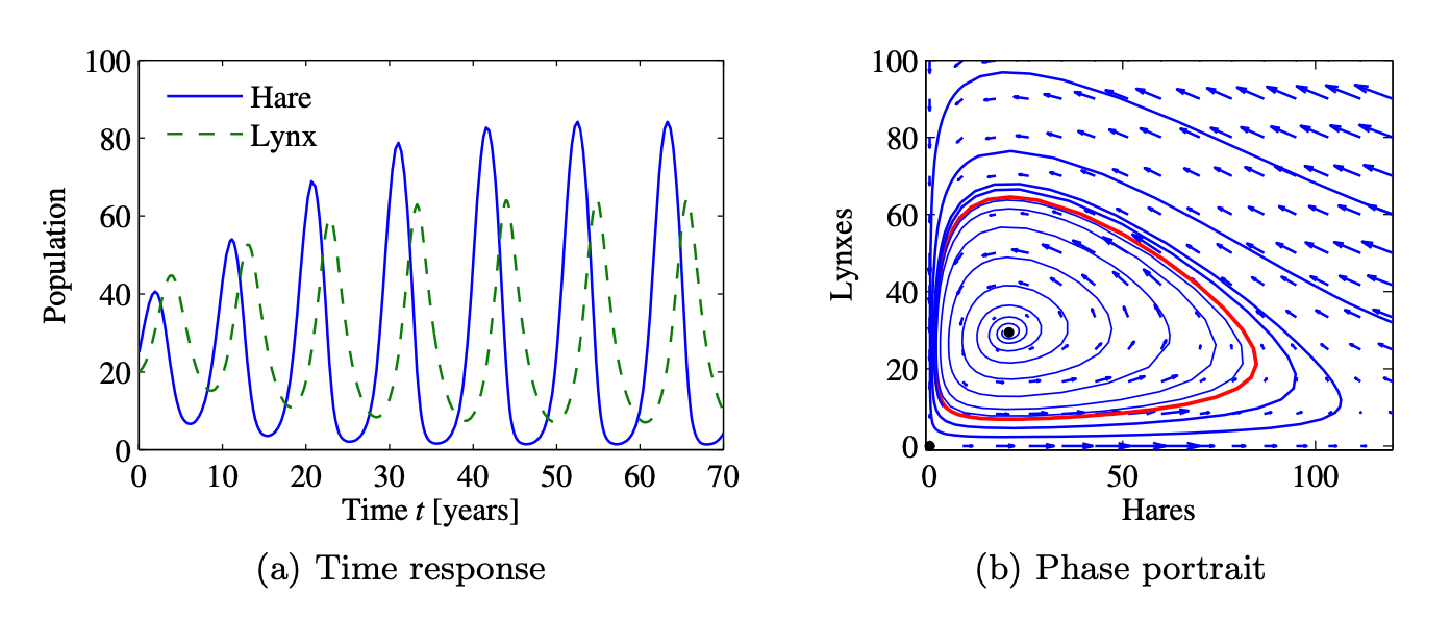
\includegraphics[width=0.8\linewidth]{figure4.20}
	\\
	\textbf{Figure 4.20:} Simulation results for the uncontrolled predator-prey system ($u=0$).
\end{figure}

\end{frame}


\begin{frame}{Example continued}
Choosing parameters $a=3.2$, $b=0.6$, $c=50$, $d=0.56$, $k=125$,  $r=1.6$, taking the growth rate for hares as the input to the system $u$ (potentially controlled by a food source for the hares), taking the number of lynxes $L$ as the output, and linearising around the equilibrium point we get 
	\[\frac{\mathrm{d}}{\mathrm{d}t}\begin{bmatrix}
		z_1 \\ z_2
	\end{bmatrix} = \begin{bmatrix}
		0.13 & -0.93 \\ 0.57 & 0
	\end{bmatrix} \begin{bmatrix}
		z_1 \\ z_2
	\end{bmatrix}  + \begin{bmatrix}
		17.2 \\ 0
	\end{bmatrix} v\]
	\[w=\begin{bmatrix}
		0& 1
	\end{bmatrix}  \begin{bmatrix}
		z_1 \\ z_2
	\end{bmatrix} \]
where $z_1=H-H_e$, $z_2=L-L_e$, and $v=u$
	
This system is reachable (by showing that the reachability matrix is full rank) and therefore we can assign the eignenvalues using state feedback

\end{frame}

\begin{frame}{Example continued}
	
	Choosing $\lambda=\begin{bmatrix}
		-0.1 & -0.2
	\end{bmatrix}$ as our desired eigenvalues, we may use the eigenvalue assignment approach to get $K=\begin{bmatrix}
		0.025 & -0.052
	\end{bmatrix}$ and $k_f=0.002$ for our gain values
	
	The resulting control law tells us how we should change the food source for the hares as a function of the current number of lynxes and hares to stabilise both populations to their equilibria
\begin{figure}
	\centering
	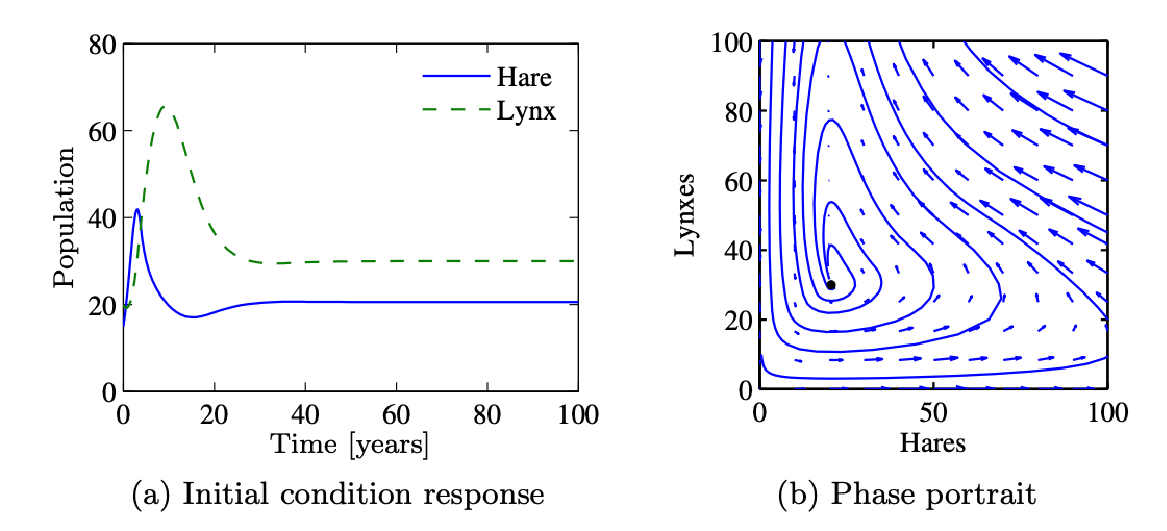
\includegraphics[width=0.8\linewidth]{figure7.7}
	\\
	\textbf{Figure 7.7:} Simulation for the controlled predator-prey system.
\end{figure}
\end{frame}


\SUMMARYFRAME
\FINALE

\end{document}
